\documentclass[a4j,titlepage]{jarticle}
\usepackage[dvipdfmx]{graphicx}
\usepackage{ascmac}
\usepackage{float}
\usepackage{amssymb}%にやりイコールを使う
\usepackage{multirow}
\usepackage{multicol}
%\usepackage{color}

\begin{document}

\title{2022 年度 3 回生前期学生実験 HW  \\ \bf team02 最終成果物のユーザーマニュアル}
% ↓ここに自分の氏名を記入
\author{最終成果物のユーザーマニュアルの作成者:植田健斗\\
グループメンバー:\\伊藤舜一郎 (学籍番号:1029-32-7548)
\\植田健斗 (学籍番号:1029-32-6498)}
\西暦
\date{提出期限:6月9日13時 提出日: \today} % コンパイル時の日付が自動で挿入される
\maketitle
\newpage

\section{概要}
授業資料の仕様を満たすプロセッサをもとにして、拡張機能の追加をしたプロセッサを設計した。
このプロセッサは、高速化を目標にして、拡張機能を追加した。
このプロセッサの実装で特に力を入れた箇所は以下の箇所である。
\begin{itemize}
\item 5段のパイプライン処理
\item 即値命令ADDIの実装
\end{itemize}

\section{性能と特長}
\subsection{動作周波数}
このプロセッサは入力CLKに40MHzのクロック信号を与えることで、FPGA上で内部的に50MHzで動作する。
\subsection{CPI}
5命令が並列処理されているときのCPIは以下のようになっている。
\begin{itemize}
\item ロード命令(LD)は1だが、ロード命令で書きこむレジスタの内容を次の命令で読み出す場合(詳しくはハザード検出ユニットを参照のこと)は2
\item 入力命令(IN)は1以上で、execボタンが押されるまでのクロック数
\item 条件分岐・無条件分岐命令はいずれも、分岐が不成立の場合は1、成立する場合は2
\item その他の命令は、すべて1
\end{itemize}
\subsection{特徴}
このプロセッサの特徴を以下に記す。
\begin{itemize}
\item 5段のパイプライン処理
\item 即値命令ADDI
\end{itemize}

\section{命令セット・アーキテクチャ}
命令セットアーキテクチャは以下の図\ref{instructionSet}のようになる。
\newpage

\begin{figure}[H]
    \begin{center}
    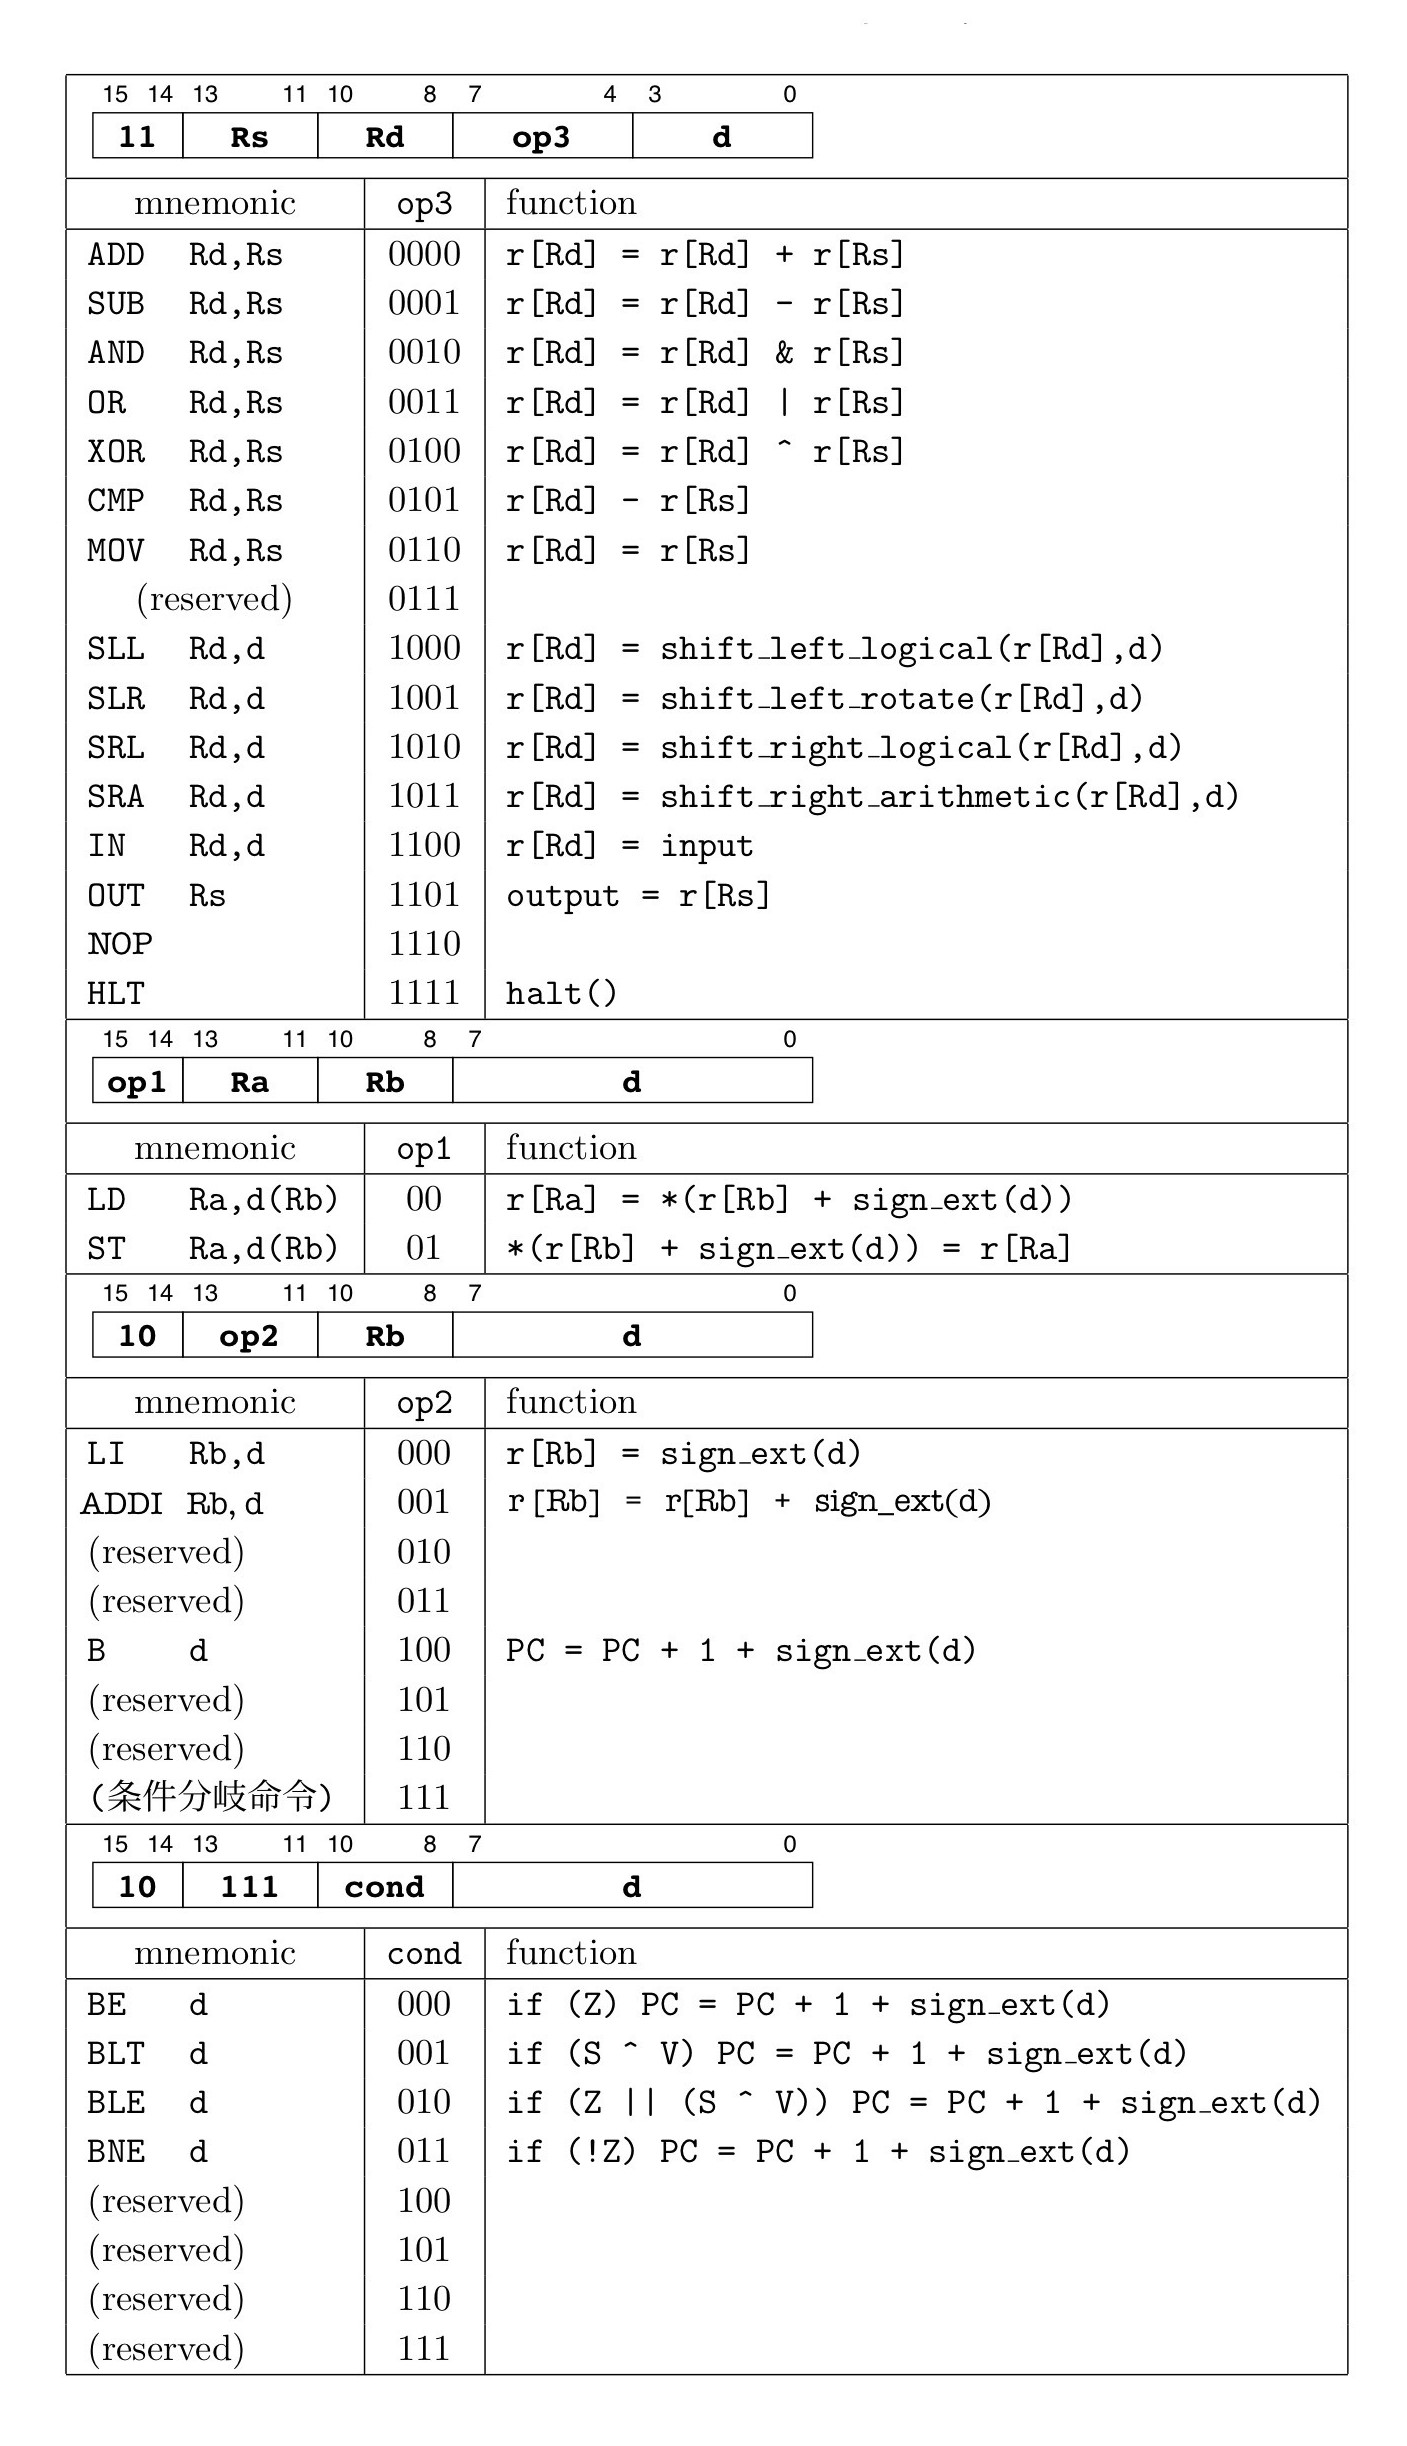
\includegraphics[scale = 0.34]{instructionSet.jpg}
    \end{center}
    \caption{命令セット・アーキテクチャ}
    \label{instructionSet}
\end{figure}

以下命令形式と各命令について、詳しく説明する。

\subsection{命令形式}
命令は全て 1 語 (16 ビット) の固定長であり,以下に示すように 4 種類の命令形式が
ある.各命令形式とフィールドの意味は以下の通りである.
\begin{enumerate}
\item 演算/入出力命令形式
\begin{description}
    \item [$I_{15:14}$ (op1)] 操作コード (11) (operation code, opcode)
    \item [$I_{13:11}$ (Rs)] ソースレジスタ番号
    \item [$I_{10:8}$ (Rd)] デスティネーションレジスタ番号
    \item [$I_{7:4}$ (op3)] 操作コード (0000 ~ 1111)
    \item [$I_{3:0}$ (d)] シフト桁数    
\end{description}
\item ロード/ストア命令形式
\begin{description}
\item [$I_{15:14}$ (op1)] 操作コード (00/01)
\item [$I_{13:11}$ (Ra)] ソース/デスティネーションのレジスタ番号
\item [$I_{10:8}$ (Rb)] ベースレジスタ番号
\item [$I_{7:0}$ (d)] 変位 (displacement)
\end{description}
\item 即値ロード/無条件分岐命令形式
\begin{description}
\item [$I_{15:14}$ (op1)]操作コード (10)
\item [$I_{13:11}$ (op2)]操作コード (000 ~ 110)
\item [$I_{10:8}$ (Rb)]ソース/デスティネーション/ベースのレジスタ番号
\item [$I_{7:0}$ (d)]即値または変位
\end{description}
\item 条件分岐命令形式
\begin{description}
\item [$I_{15:14}$ (op1)]操作コード (10)
\item [$I_{13:11}$ (op2)]操作コード (111)
\item [$I_{10:8}$ (cond)]分岐条件
\item [$I_{7:0}$ (d)]変位
\end{description}
\end{enumerate}

\subsection{算術演算(授業資料をそのまま掲載)}
レジスタ Rd と Rs の加算 (ADD: add) または減算 (SUB: subtract) の結果を Rd に格納し,条
件コードを設定する.条件コード C には最上位ビットからの桁上げが設定される.

\subsection{論理演算(授業資料をそのまま掲載)}
レジスタ Rd と Rs の,ビットごとの論理積 (AND: and), 論理和 (OR: or),または排他的論理
和 (XOR: exclusive-or) の結果を Rd に格納し,条件コードを設定する.但し条件コード C は
演算結果に関わらず 0 となる.

\subsection{比較演算 (CMP: compare)(授業資料をそのまま掲載)}
レジスタ Rd から Rs を減算し,結果に基づく条件コード設定のみを行う.条件コード C には
最上位ビットからの桁上げが設定される.

\subsection{移動演算 (MOV: move)(授業資料をそのまま掲載)}
レジスタ Rd に Rs の値を単に格納し,Rd の値に基づき条件コードを設定する.但し条件コー
ド C は Rs の値に関わらず 0 となる.

\subsection{シフト演算(授業資料をそのまま掲載)}
レジスタ Rd の値を,以下のようにシフトした値を Rd に格納し,条件コードを設定する.

\begin{description}
\item [SLL (shift left logical)] 左論理シフト.左シフト後,空いた部分に 0 を入れる.
\item [SLR (shift left rotate)] 左循環シフト.左シフト後,空いた部分にシフトアウトされたビット列を入れる.
\item [SRL (shift right logical)] 右論理シフト.右シフト後,空いた部分に 0 を入れる.
\item [SRA (shift right arithmetic)] 右算術シフト.右シフト後,空いた部分に符号ビットの値を入れる.
\end{description}

シフト桁数は即値 d (0 ~ 15) である.また条件コード C には,シフト桁数が 0 の時または
SLR では 0 が,それ以外では最後にシフトアウトされたビットの値が設定される.条件コー
ド V は常に 0 が設定される.

\subsection{ロード/ストア命令(授業資料をそのまま掲載)}
ロード命令 (LD: load) とストア命令 (ST: store) の機能を説明する.ソース/デス
ティネーションは,フィールド Ra で指定されたレジスタ Ra である.また実効アドレスはベース
レジスタアドレス指定により,フィールド Rb で指定されたレジスタ Rb と,フィールド d を符号
拡張した sign ext(d) を加算して求める.
ロード命令のSZCVフラグは未定義である。また、ストア命令のSZCVフラグについては
メモリに格納するデータが
正のときSZCV=0000、負のときSZCV=1000、0のときSZCV=0100となるようにSZCVフラグを設定される。



\subsection{即値ロード/無条件分岐命令(授業資料をそのまま掲載)}
SIMPLE の即値ロード命令 (LI: load immediate) と,無条件分岐命令 (B: branch) の機能を以下
に示す.即値ロード命令のSZCVフラグについては即値dを符号拡張した値が
正のときSZCV=0000、負のときSZCV=1000、0のときSZCV=0100となるようにSZCVフラグを設定される。
\begin{description}
\item [LI] 即値 sign ext(d) をレジスタ Rb に格納する.
\item [B] d を符号拡張した値を変位として,PC 相対アドレス指定による分岐を行う.
\end{description}

\subsection{条件分岐命令(授業資料をそのまま掲載)}
SIMPLE の条件分岐命令は,フィールド cond で定められる分岐条件が成り立
てば PC 相対アドレスによる分岐を行ない,成り立たなければ単に次の命令に移行する.各命令の
分岐条件は以下の通り.
\begin{description}
\item [BE (branch on equal-to)] 条件コード Z が 1
\item [BLT (branch on less-than)] 条件コード S と V の XOR(S \^ V) が 1
\item [BLE (branch on less-than or equal-to)] Z または (S \^ V) が 1
\item [BNE (branch on not-equal-to)] 条件コード Z が 0
\end{description}

\subsection{IN命令}
IN命令が呼ばれると実行を一時的に中断し、外部入力で入力された値をうけとる。
実行の中断中に16個のディップスイッチを変更し、16bitの値を設定し、
execボタンを押すことでexecボタンが押された時のディップスイッチを用いて表現された値を入力として受け取り、
実行を再開するようにした。その値をIN命令中で指定した番号のレジスタに格納する。
IN命令のSZCVフラグは未定義である。

\subsection{OUT命令}
OUT命令が呼ばれると、フェーズがp3の時に外部出力にRsフィールドで指定したレジスタの中身が渡される。
外部出力では7SEG-LEDを4つ用いて16進数表示で16bitのデータを表示する。
また、過去16回のOUT命令で出力されたデータを保持し、7SEG-LEDに表示する。
OUT命令のときのSZCVフラグについてはOUT命令により出力されるデータが、
正のときSZCV=0000、負のときSZCV=1000、0のときSZCV=0100となるようにSZCVフラグを設定される。

\subsection{HLT命令}
命令の実行を中断するための命令である。内部的にはexecボタンが押されたのと同じ動作をする。
HLT命令が呼ばれた後に、execボタンを押すとメモリ上でHLT命令の次の命令から命令の実行を再開する。
HLT命令が呼ばれた後、HLT命令の次の番地に命令を書いていない場合に、execボタンを押すと
未定義動作を引き起こす可能性があるので、注意が必要である。

\subsection{NOP命令(non operation)}
レジスタ・メモリ書き込み、外部入出力などの動作を、何も行わない命令である。
この命令はハードウェアで、リセットの動作をする際や、パイプラインストールの際に
何もしない命令が必要であるためにある。機器の初期化の際には、
resetボタンが押されるとInstruction Registerの値は2'b 1100000011100000となり、NOP命令の値に設定される。
なお “(reserved)” と記された命令は何の動作もせず,単に次の命令に移行する.

\subsection{ADDI命令(add immediate)}
Rbフィールドで指定したレジスタの中身を読み出し、命令の下8bitで指定した符号付きの値dを足し合わせる。
足し合わせた値をRbフィールドで指定したレジスタに格納する。Rbフィールドの値により、条件コードが
設定される。条件コード C には最上位ビットからの桁上げが設定される。

\section{構造と動作}

\subsection{構造}

現状のプロセッサの構造は以下の図\ref{structure0506}のようになる。

\begin{figure}[H]
    \begin{center}
     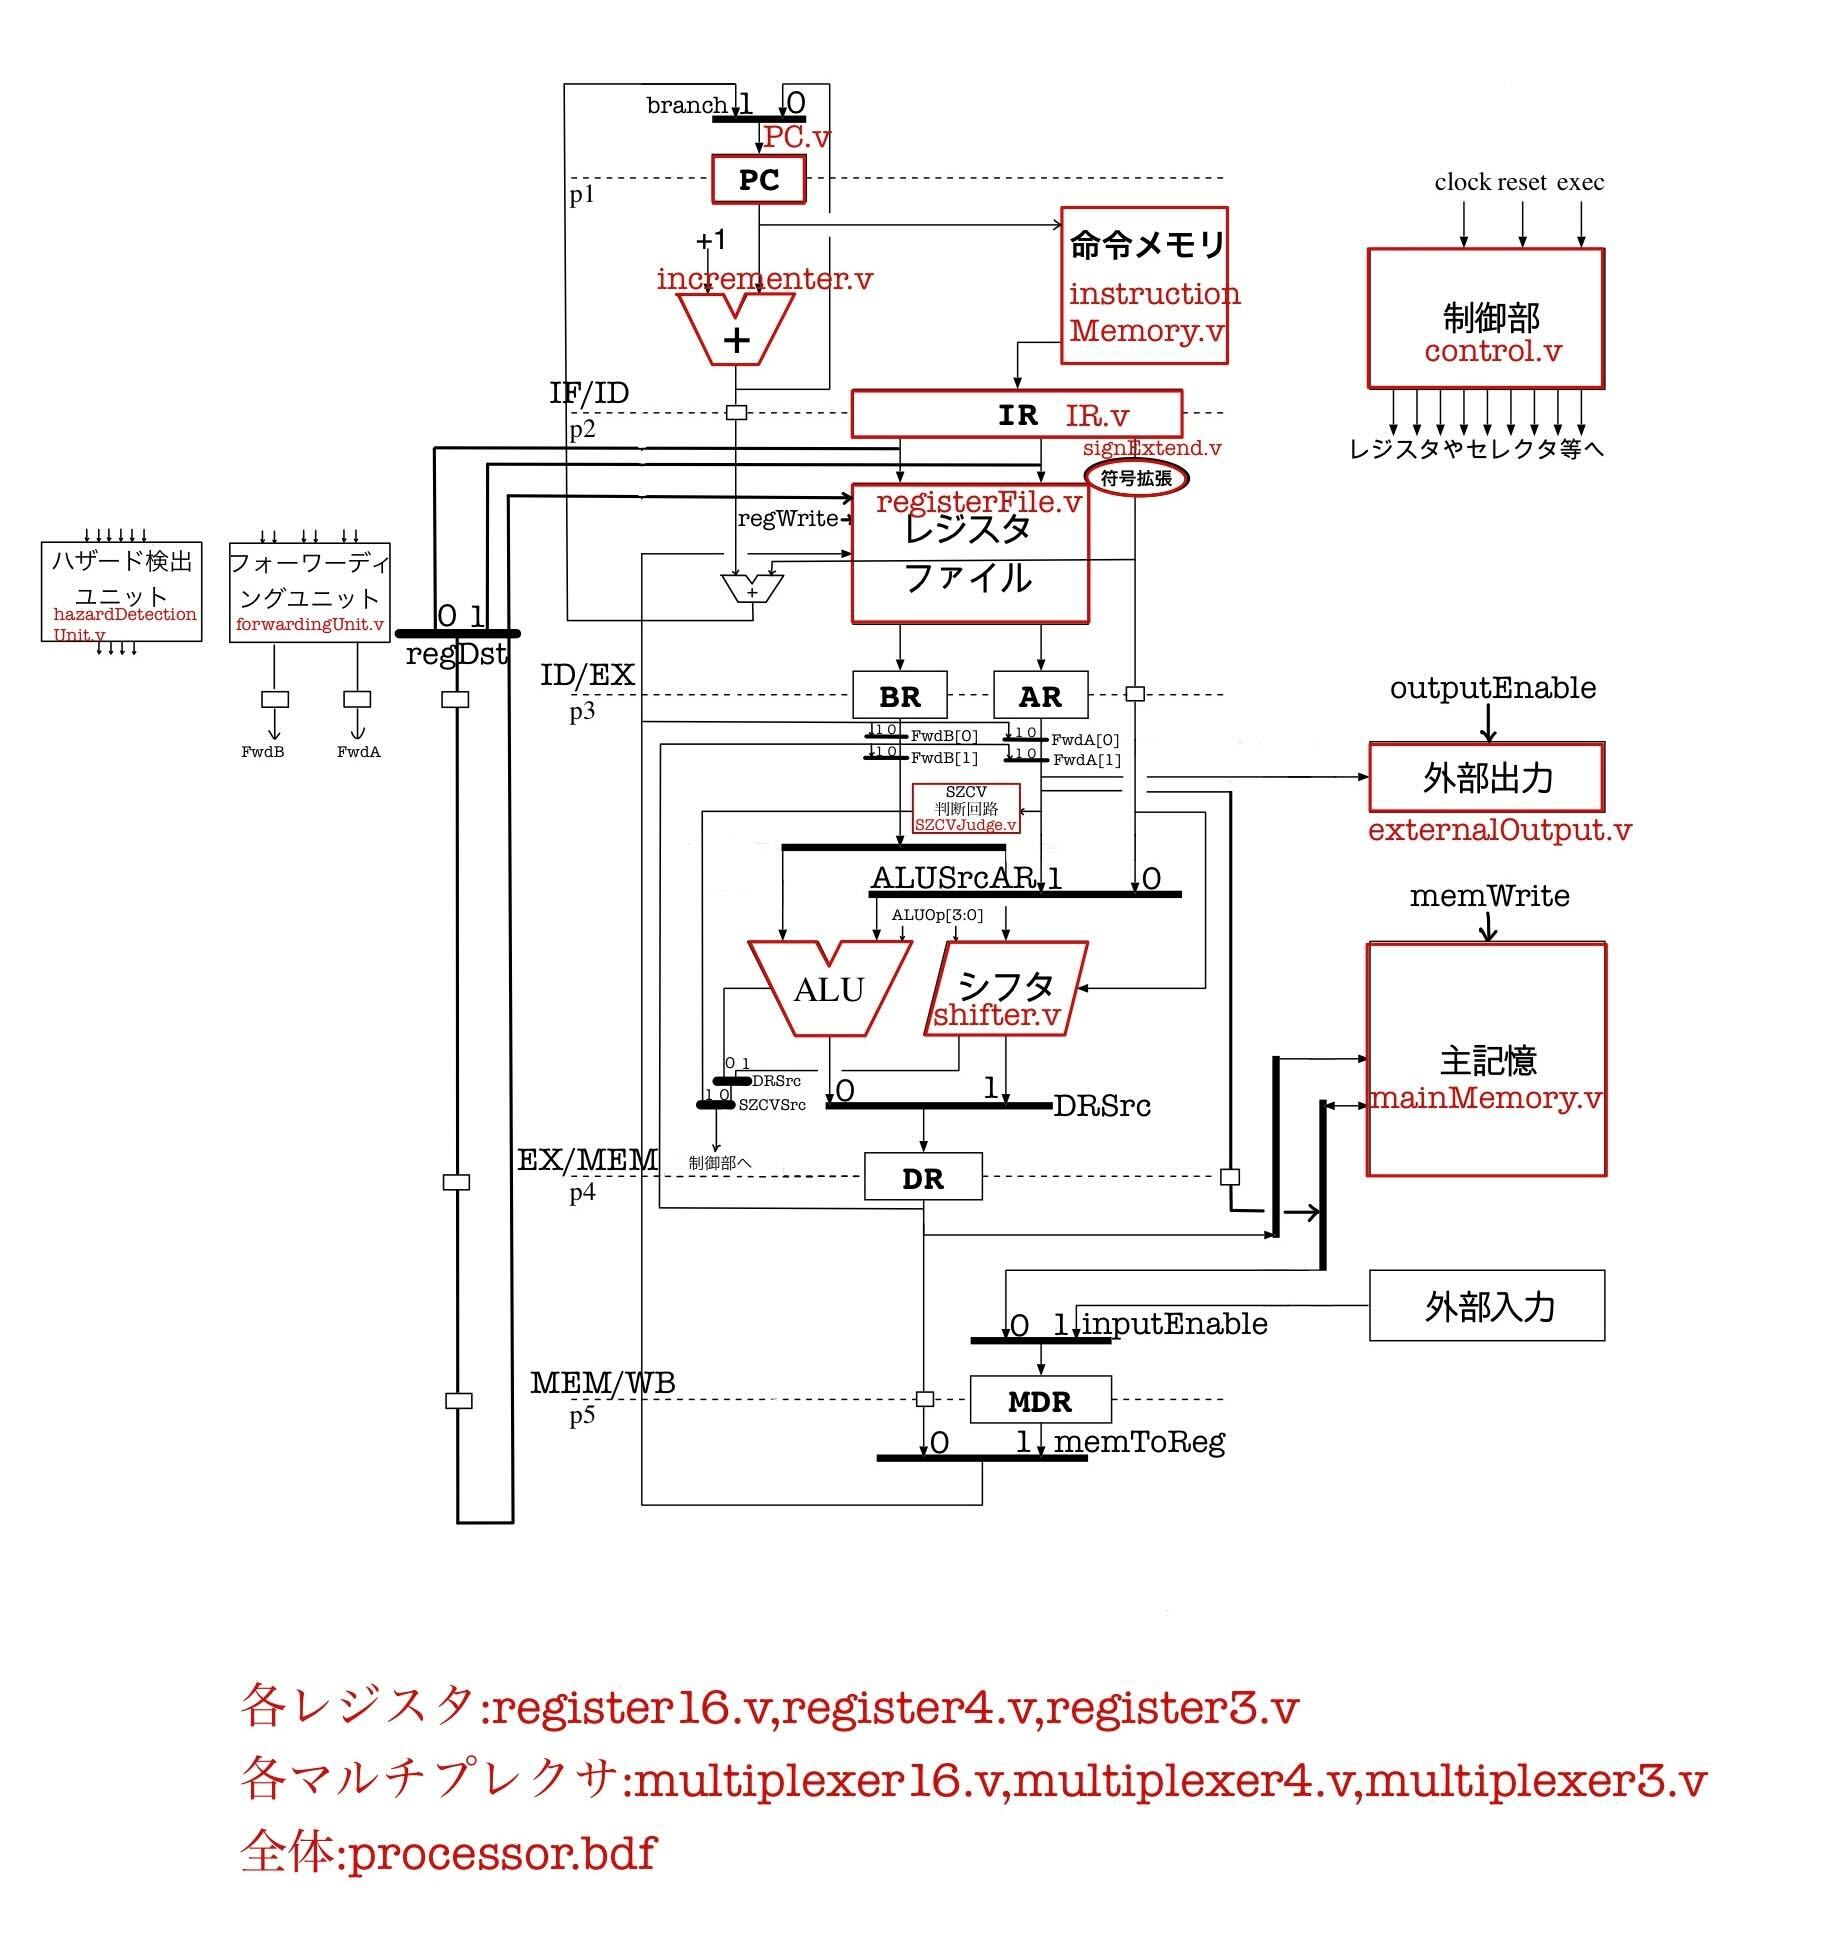
\includegraphics[scale = 0.22]{structure0526.jpg}
     \end{center}
     \caption{プロセッサの構造(最終段階)}
     \label{structure0506}
 \end{figure}

パイプライン化に伴い必要な構造を以下で示す。

\begin{itemize}
\item メモリを命令メモリとデータメモリに分け、構造ハザードを防いでいる。(ハーバードアーキテクチャ)
\item ALUとは別にアドレス計算用の加算器を用意し、アドレス計算と演算の際のALUでの構造ハザードを防いでいる。
\item 各フェーズの間でデータを送る際に、配線ではなくレジスタを用意し、
フェーズ間での制御信号やデータの受け渡しを行う。
\item MEMフェーズもしくはWBフェーズから、ALUのあるEXフェーズに、
データのフォーワーディングを行うフォーワーディングユニットを追加した。
\item IDフェーズでレジスタを読み込みと、WBフェーズでレジスタ書き込みを
同じクロック周期内で同じレジスタに対して行うときに、レジスタに書きこもうとする
データをレジスタから読み出されるように、レジスタファイルの設計をした。
\item ロード命令(LD)や入力命令(IN)でレジスタに値を格納し、
その次の演算命令でその値を読み出そうとすることを考える。レジスタから読み出しをする際に
レジスタに書きこむ値がまだわからないため、読み出せない問題(パイプラインストール)が発生する。
パイプラインストールが起こったときに、ロード命令(LD)や入力命令(IN)の次に
NOP命令を入れて、データハザードを防ぐ、ハザード検出ユニットを追加する。
\item 分岐が成立した際に、不成立分岐予測により読み込んだ次の命令を、
フラッシュ(NOP命令に置き換える)する機能を、
ハザード検出ユニットに追加する。
\item メモリ読み出しを行っているときに1になる信号であるmemRead信号を追加し、
パイプラインストールの判定に用いた。
\end{itemize}

これらの構造がパイプライン化のために必要な構造である。
パイプライン化により、プロセッサ全体の外部仕様は変えずに、処理の高速化を行う。

\subsection{動作}

このプロセッサは5フェーズに処理をわけ、それぞれを
p1(IF),p2(ID),p3(EX),p4(MEM),p5(WB)というフェーズとする。
p1からp5のそれぞれを並列実行するパイプライン処理を行うようにした。
それぞれのフェーズ間、つまり、図\ref{structure0506}の破線上に
フェーズ間のデータの受け渡しを行うパイプラインレジスタを配置する。
クロックの立ち上がりごとにパイプラインレジスタの値は更新され、
それぞれのフェーズにおかれた組み合わせ回路の入力となる。
その組み合わせ回路からの出力が、次のフェーズの間のパイプラインレジスタに
入力され、次のクロックの立ち上がりにパイプラインレジスタの値が更新される。
これを繰り返すことで、それぞれの命令は原則1クロックあたり1フェーズずつ進む。
各命令は、1つのフェーズ内の回路のみを使うため、
命令の処理をフェーズごとに独立に行うことができ、
それにより、5つの命令を並列実行している。

このプロセッサに用いられるそれぞれのレジスタはイネーブル信号を入力として受け取る。
レジスタのイネーブル信号とは、クロックの立ち上がりでかつ、
レジスタのイネーブル信号が1であるときのみ、レジスタの中身が書き変わり、
それ以外はレジスタの中身は変わらないような信号である。

このプロセッサは制御部内にSystemRunningという1bitのレジスタをもっており、
そのレジスタの値が0のときにSystemRunningレジスタ以外の
すべてのレジスタのイネーブル信号が0になるようになっている。

execボタンを押されると、このSystemRunningの反転が行われる。
これによりexecボタンを押すたびに実行停止・再開ができる。

resetボタンを押すと、以下のことがすべて行われる。
\begin{itemize}
\item IRにNOP命令を表す命令コード2'b 1100000011100000が格納される。
\item PCに0が格納される。
\item 外部出力の過去の出力履歴がクリアされる。
\item レジスタファイルの内部のレジスタに0が格納される。
\item SystemRunningに0が格納される。
\item 制御信号を格納するレジスタで、
レジスタ・メモリ書き込み、入出力、メモリ読み出しのための制御信号
(つまり制御信号outputEnable,memRead,inputEnable,memWrite,branch,regWrite)を
0にし、書き込み、入出力、ハザード検出が行われないようにする。
\end{itemize}
これによりresetボタンを押すことで機器を初期状態にし、実行待機状態にすることができる。
この状態でexecボタンを押すとメモリの0番地から順に命令が実行される。

FPGAにプログラムをダウンロードした後にexecボタンを押さなければ、
命令が実行されないことに注意が必要である。

また、HLT命令は、execボタンが押されたのと同じ動作をするので、HLT命令の
後ろに命令を記述しておいた場合、HLT命令で実行を中断し、
そこから、execボタンを押すと実行を再開できる。
これを用いると、OUT命令の次にHLT命令を
実行することで、OUT命令のたびに一時停止するので、
出力を確認してからexecボタンを押し実行を再開することができる。

ただ、HLT命令の次の番地に命令を記述していない場合に、HLT命令で止まった後、
execボタンが押されると未定義動作を引き起こすので注意が必要である。

\subsection{ピン配置}
ピン配置は以下の図\ref{UI}のようになる。OUT命令、IN命令での入出力は、それぞれ7SEG-LEDとディップスイッチをもちいてやっている。

\begin{figure}[H]
    \begin{center}
    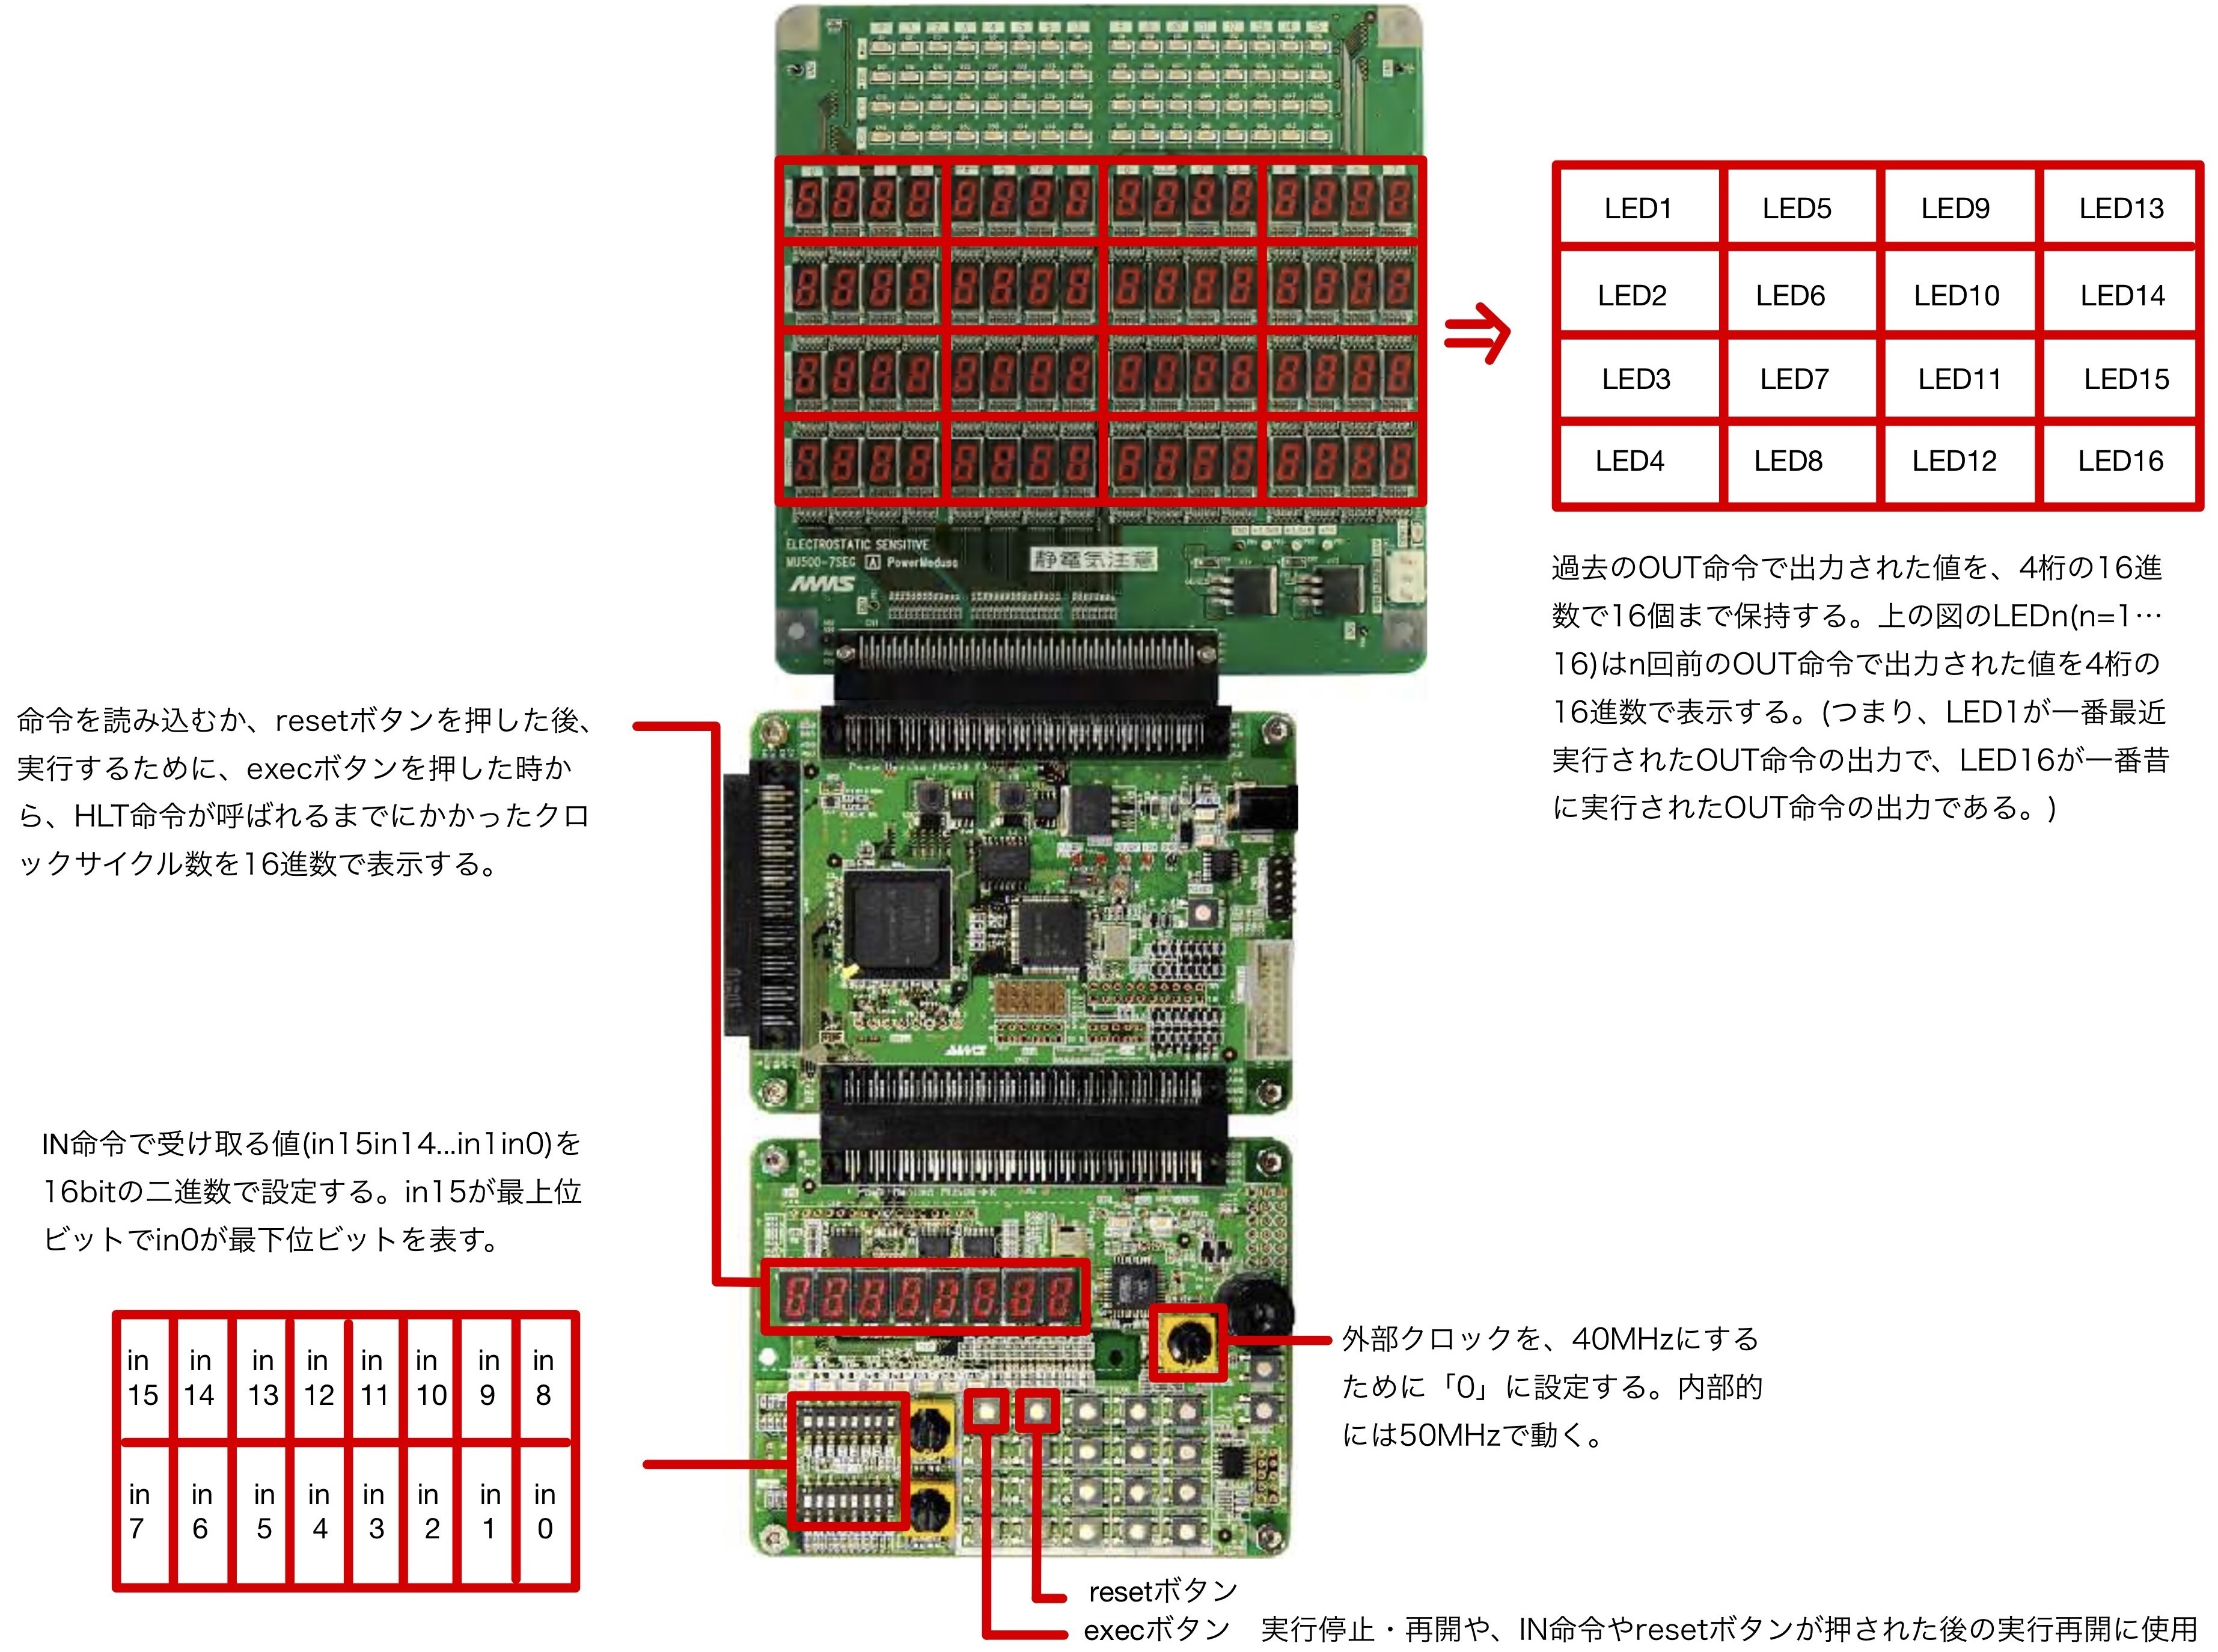
\includegraphics[scale = 0.12]{UI.jpg}
    \end{center}
    \caption{ピン配置}
    \label{UI}
\end{figure}


\end{document}
